\documentclass[FU]{matheon-poster}
% load some useful latex symbols:
\usepackage{latexsym}
% define names for even more symbols:
\usepackage{textcomp}
% define several useful macros for typesetting mathematics:
\usepackage{amsmath,amssymb}
% load mathematic fonts:
\usepackage{amsfonts}
% for typesetting paragraphs in a special form:
\usepackage{shapepar}
% for setting the examples
\usepackage{alltt}
% for extended possibilities in setting arrays and tables
\usepackage{array}
% For typesetting boxes
\usepackage[oldboxesoff]{poster-boxes}

\usepackage{color}
\usepackage{tabularx}
\usepackage{multirow}
\usepackage{enumitem}

\newcolumntype{C}{>{\centering\arraybackslash}X}
%\newcommand{\shortitemize}{itemsep=0.25\itemsep,parsep=0.25\parsep,topsep=0.25\topsep,partopsep=0.25\partopsep}
\newenvironment{shortitemize}{\begin{itemize}[itemsep=0.25\itemsep,parsep=0.25\parsep,topsep=0.25\topsep,partopsep=0.25\partopsep]}{\end{itemize}}

% You can define colors as follows:
\definecolor{light-red}{rgb}{1, 0.59, 0.59}
\newcommand{\leftcolspace}{0.025\contentswidth}
\newcommand{\leftcolwidth}{0.6\contentswidth}
\newcommand{\rightcolspace}{0.65\contentswidth}
\newcommand{\rightcolwidth}{0.325\contentswidth}
\newcommand{\contwidth}{0.95\contentswidth}


\definecolor{question}{rgb}{0.29,0.29,0.73}

%Mathcal
\newcommand{\T}{\mathcal{T}}
\newcommand{\E}{\mathcal{E}}
\newcommand{\K}{\mathcal{K}}
\newcommand{\M}{\mathcal{M}}
\newcommand{\I}{\mathcal{I}}
\newcommand{\J}{\mathcal{J}}
\newcommand{\C}{\mathcal{C}}
\newcommand{\A}{\mathcal{A}}

%Mathbb
\newcommand{\R}{\mathbb{R}}
\newcommand{\N}{\mathbb{N}}

\DeclareMathOperator{\res}{Res}
\DeclareMathOperator{\osc}{osc}
\renewcommand{\div}{\textrm{div}}
\newcommand{\Jump}[1]{\lbrack #1 \rbrack \!\cdot\! \nu_E}
\newcommand{\jump}[1]{\lbrack #1 \rbrack}

\newcommand{\bnorm}[1]{\lVert #1 \rVert}
\newcommand{\anorm}[1]{\lvert\!\lvert\!\lvert#1 \rvert\!\rvert\!\rvert}
\newcommand{\norm}[2]{\lVert #1 \rVert_{#2}}
\newcommand{\Norm}[2]{\big\lVert #1\big\rVert_{#2}}
\newcommand{\snorm}[2]{\lvert #1 \rvert_{#2}}
\newcommand{\abs}[1]{\lvert #1 \rvert}

\newcommand{\hmax}{\norm{h_\ell}{L^\infty(\Omega)}}


\makeatletter
  \newcommand\huuge{\@setfontsize\huuge{18.5pt}{20}}
\makeatother

%---------------------------------------------------------------------------
\begin{document}
\titlebox{}
{}
{\Huge SIAM Student Chapter at TU Delft}
{}


\begin{pspicture}(0,0)(\contentswidth,\contentsheight)

\rput[tl](\leftcolspace,231mm){
  \posterroundedtabshadowbox{white}{\fbsdefault}{\leftcolwidth}{\large Society for Industrial and Applied Mathematics (SIAM)}{
    \small\raggedright
\textbf{\underline{Geo-scientists want to analyze the earth interior:}}
\smallskip
\begin{shortitemize}
 \item The earth interior consists of several layers with different physical properties,
 \item Seismic exploration: send sound waves into the earth and analyze their reflection behavior,
 \item The properties of an oil reservoir can be derived by matching experimental and nu\-me\-ri\-cal results within an optimization loop.
\end{shortitemize}
  }
}

\rput[tl](\leftcolspace,187.5mm){
  \posterroundedtabshadowbox{white}{\fbsdefault}{\leftcolwidth}{\large SIAM Student Chapters}{
    \small\raggedright
    Text...
    \smallskip
  \begin{shortitemize}
    \item The earth interior consists of several layers with different physical properties,
    \item Seismic exploration: send sound waves into the earth and analyze their reflection behavior,
    \item The properties of an oil reservoir can be derived by matching experimental and nu\-me\-ri\-cal results within an optimization loop.
  \end{shortitemize}
  }
}

\rput[tl](\leftcolspace,143mm){
  \posterroundedtabshadowbox{white}{\fbsdefault}{\leftcolwidth}{\large Chapter activities}{
    \small\raggedright
    Text...
    \smallskip
  \begin{shortitemize}
    \item The earth interior consists of several layers with different physical properties,
    \item Seismic exploration: send sound waves into the earth and analyze their reflection behavior,
    \item The properties of an oil reservoir can be derived by matching experimental and nu\-me\-ri\-cal results within an optimization loop.
    \item The properties of an oil reservoir can be derived by matching experimental and nu\-me\-ri\-cal results within an optimization loop.
    \item The properties of an oil reservoir can be derived by matching experimental and nu\-me\-ri\-cal results within an optimization loop.
   \end{shortitemize}
  }
}

\rput[tl](\leftcolspace,82mm){
  \posterroundedtabshadowbox{white}{\fbsdefault}{13cm}{\large Group picture}{
  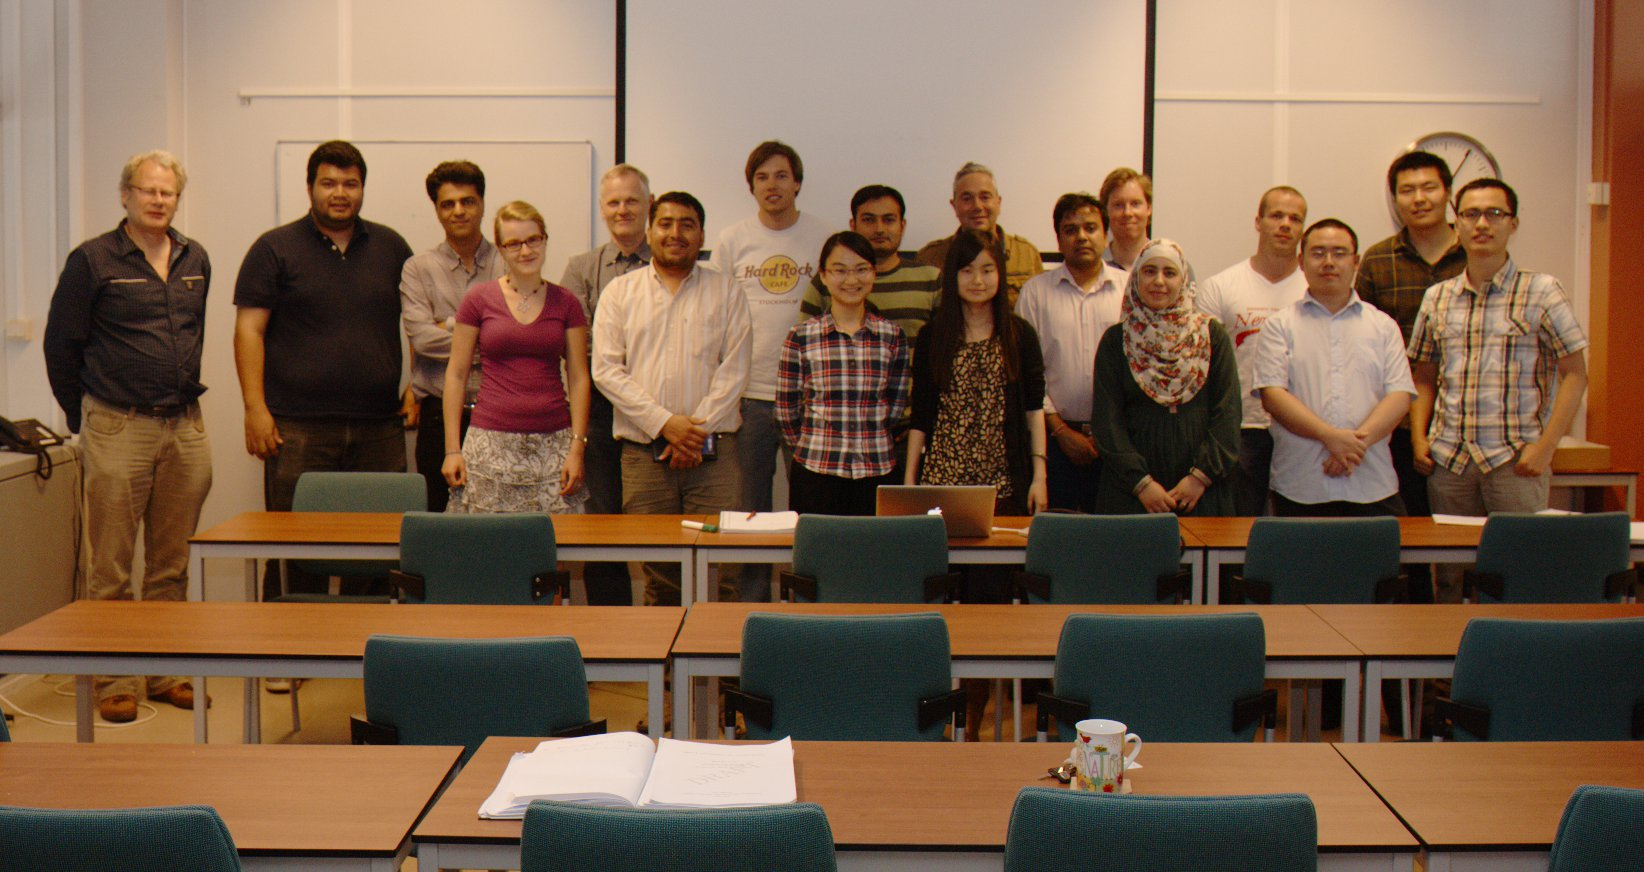
\includegraphics[scale=0.2]{group}} 
}

\rput[tl](141mm,231mm){
  \posterroundedtabshadowbox{white}{\fbsdefault}{6cm}{\large SIAM chapters in Europe}{
  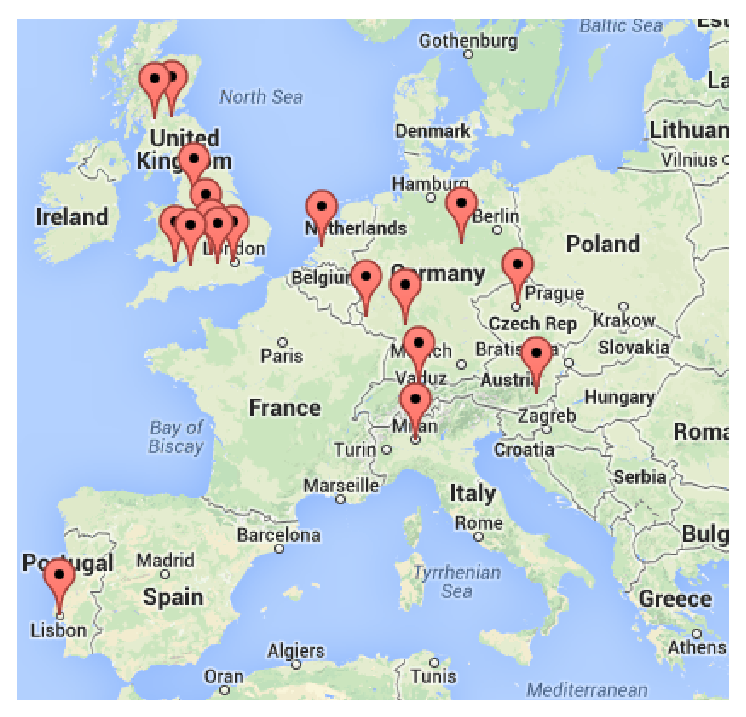
\includegraphics[scale = 0.38]{siam_map_with_delft2}} 
}

\rput[tl](141mm,143mm){
  \posterroundedtabshadowbox{white}{\fbsdefault}{6cm}{\large Who are we ?}{
  The Chapter at TU Delft has been founded in 2014. 
\smallskip
  \begin{shortitemize}
    \item President:
    \item Vice-president:
    \item Secretary and Treasurer: Thea Vuik
    \item ... and many more ;-)
  \end{shortitemize}
}}

\rput[tl](141mm,82mm){
\posterroundedtabshadowbox{white}{\fbsdefault}{6cm}{\large Contact us:}{
We are happy if...
\smallskip
  \begin{shortitemize}
    \item Webpage:
    \item email:
    \item Twitter:
    \item LinkedIn:
    \item Facebook:
  \end{shortitemize}
  \vspace{0.3cm}
\centering

\includegraphics[scale=0.4]{qrcode}
}
}

\end{pspicture}
\end{document}
